\documentclass[10pt,a4paper]{article}
\usepackage[utf8]{inputenc}
\usepackage[english]{babel}
\usepackage{amsmath}
\usepackage{amsfonts}
\usepackage{amssymb}
\usepackage{natbib}
\usepackage{graphicx}
\usepackage{cleveref}
\usepackage{enumitem}
\usepackage{listings}
%\usepackage[minionint,frenchmath,mathlf]{MinionPro}
%\usepackage[toc, eqno, enum]{tabfigures}
%\figureversion{lf,tab}
\renewcommand{\familydefault}{\sfdefault}
\usepackage{helvet}
\usepackage{sfmath}
\usepackage[font={small,it}]{caption}
\parindent 0pt
\parskip 12pt
\setcounter{tocdepth}{2}
\setcounter{section}{-1}
\lstset{basicstyle=\ttfamily\small, columns=flexible, breaklines=true}

\begin{document}

\author{Bernhard Bauer-Marschallinger}
\title{\textbf{The Equi7 Grid -- V13} \\ \vspace{10 mm} \Large \textbf{\textit{Grid and Tiling Definition Document -- Issue 0.1}}}
\maketitle

%\begin{figure}[hbtp]
%\centering
%\includegraphics[width=1.0\textwidth]{frontpagefigur}
%\end{figure}

\newpage

\parskip 4pt
\tableofcontents

\newpage

\section*{Document History}

\begin{tabular}{llll}
\hline 
\textbf{Issue} & \textbf{Date} & \textbf{Author} & \textbf{Changes} \\ 
\hline 
0.1 & 2015-03-16 & Bernhard Bauer-M. & adopted for Equi7 V13 \\ 
\hline 
\end{tabular} 

\newpage

\section{Preamble}
\label{sec:preamble}

\subsubsection*{Content of Document}
This document describes the design, realisation and software of the Equi7 Grid. This grid was developed at the Department of Geodesy and Geoinformation at the TU~Wien is aimed to use for high resolution remote sensing data. 

\subsubsection*{Scientific Basis}
Detailed information on the scientific background is published under: \\
\textit{B. Bauer-Marschallinger, D. Sabel, W. Wagner: \textbf{Optimisation of global grids for high-resolution remote sensing data.} Computers \& Geosciences, 72 (2014), 84 - 93, DOI: 10.1016/j.cageo.2014.07.005}

\begin{lstlisting}
http://www.sciencedirect.com/science/article/pii/S0098300414001629
\end{lstlisting}

\subsubsection*{Acknowledgements}
This work is the result from efforts spent during ongoing developments carried out at TU Wien across a number of projects and by various staff members. In the coarse of these developments of data processing and handling capacities, profound expertise on spatial referencing of remote sensing data was built up at the TU Wien group. Thanks to FFG, time was found to craft this design document. The major work on the scientific background was carried out in the \textit{Soil Moisture Data Cubes} project. Rendering the grid operational was done in the \textit{Prepare4EODC-Water} project.

\textit{This work has received funding from the Austrian research funding association (FFG) under the scope of the ASAP 9 program within the research project \#840114, Soil Moisture Data Cubes and under the scope of the ASAP 10 program within the research project \#344350, Prepare4EODC-Water.}

\subsubsection*{License}
The Equi7 Grid V13, its software, source files and documentation are licensed under the Creative Commons Attribution-NoDerivatives 4.0 International License. To view a copy of this license, visit

\begin{lstlisting}
http://creativecommons.org/licenses/by-nd/4.0/
\end{lstlisting}

\begin{figure}[hbtp]
\centering

\includegraphics[width=0.2\textwidth]{cc_by-nd}
\end{figure}

\newpage

\parskip 10pt

\section{Overview}
\label{sec:overview}

\subsection{Rationale}
Upcoming remote sensing systems onboard satellites will generate unprecedented volumes of spatial data, hence challenging processing facilities in terms of storage and processing capacities. Thus, an efficient handling of remote sensing data is of vital importance, demanding a well-suited definition of spatial grids for the data's storage and manipulation. With a suitable grid definition, one can cut down processing time, hard disk volumes, and signal distortions stemming from geometric manipulations.

For high-resolution image data, regular grids defined by map projections have been identified as practicable, cognisant of their drawbacks due to geometric distortions. The Equi7 Grid uses the Azimuthal Equidistant Projection that minimises those distortions in the sense of remote sensing and raster imagery.

Further information on the scientific aspect of grid definitions and their suitability to high resolution remote sensing can be found in \cite{Bauer-Marschallinger2014}.

\subsection{Key Facts}
The Equi7 Grid is a spatial reference system for the entire Earth and consists of seven planar subgrids for each continent (Figure \ref{fig:7cont}). The coordinates are defined by individual realisations of the Equidistant Azimuthal projection and are referenced to the ellipsoidal WGS84 datum. The Equi7 Grid is designed to handle efficiently the archiving, processing and display of high resolution remote sensing data.

\begin{figure}[hbtp]
\centering
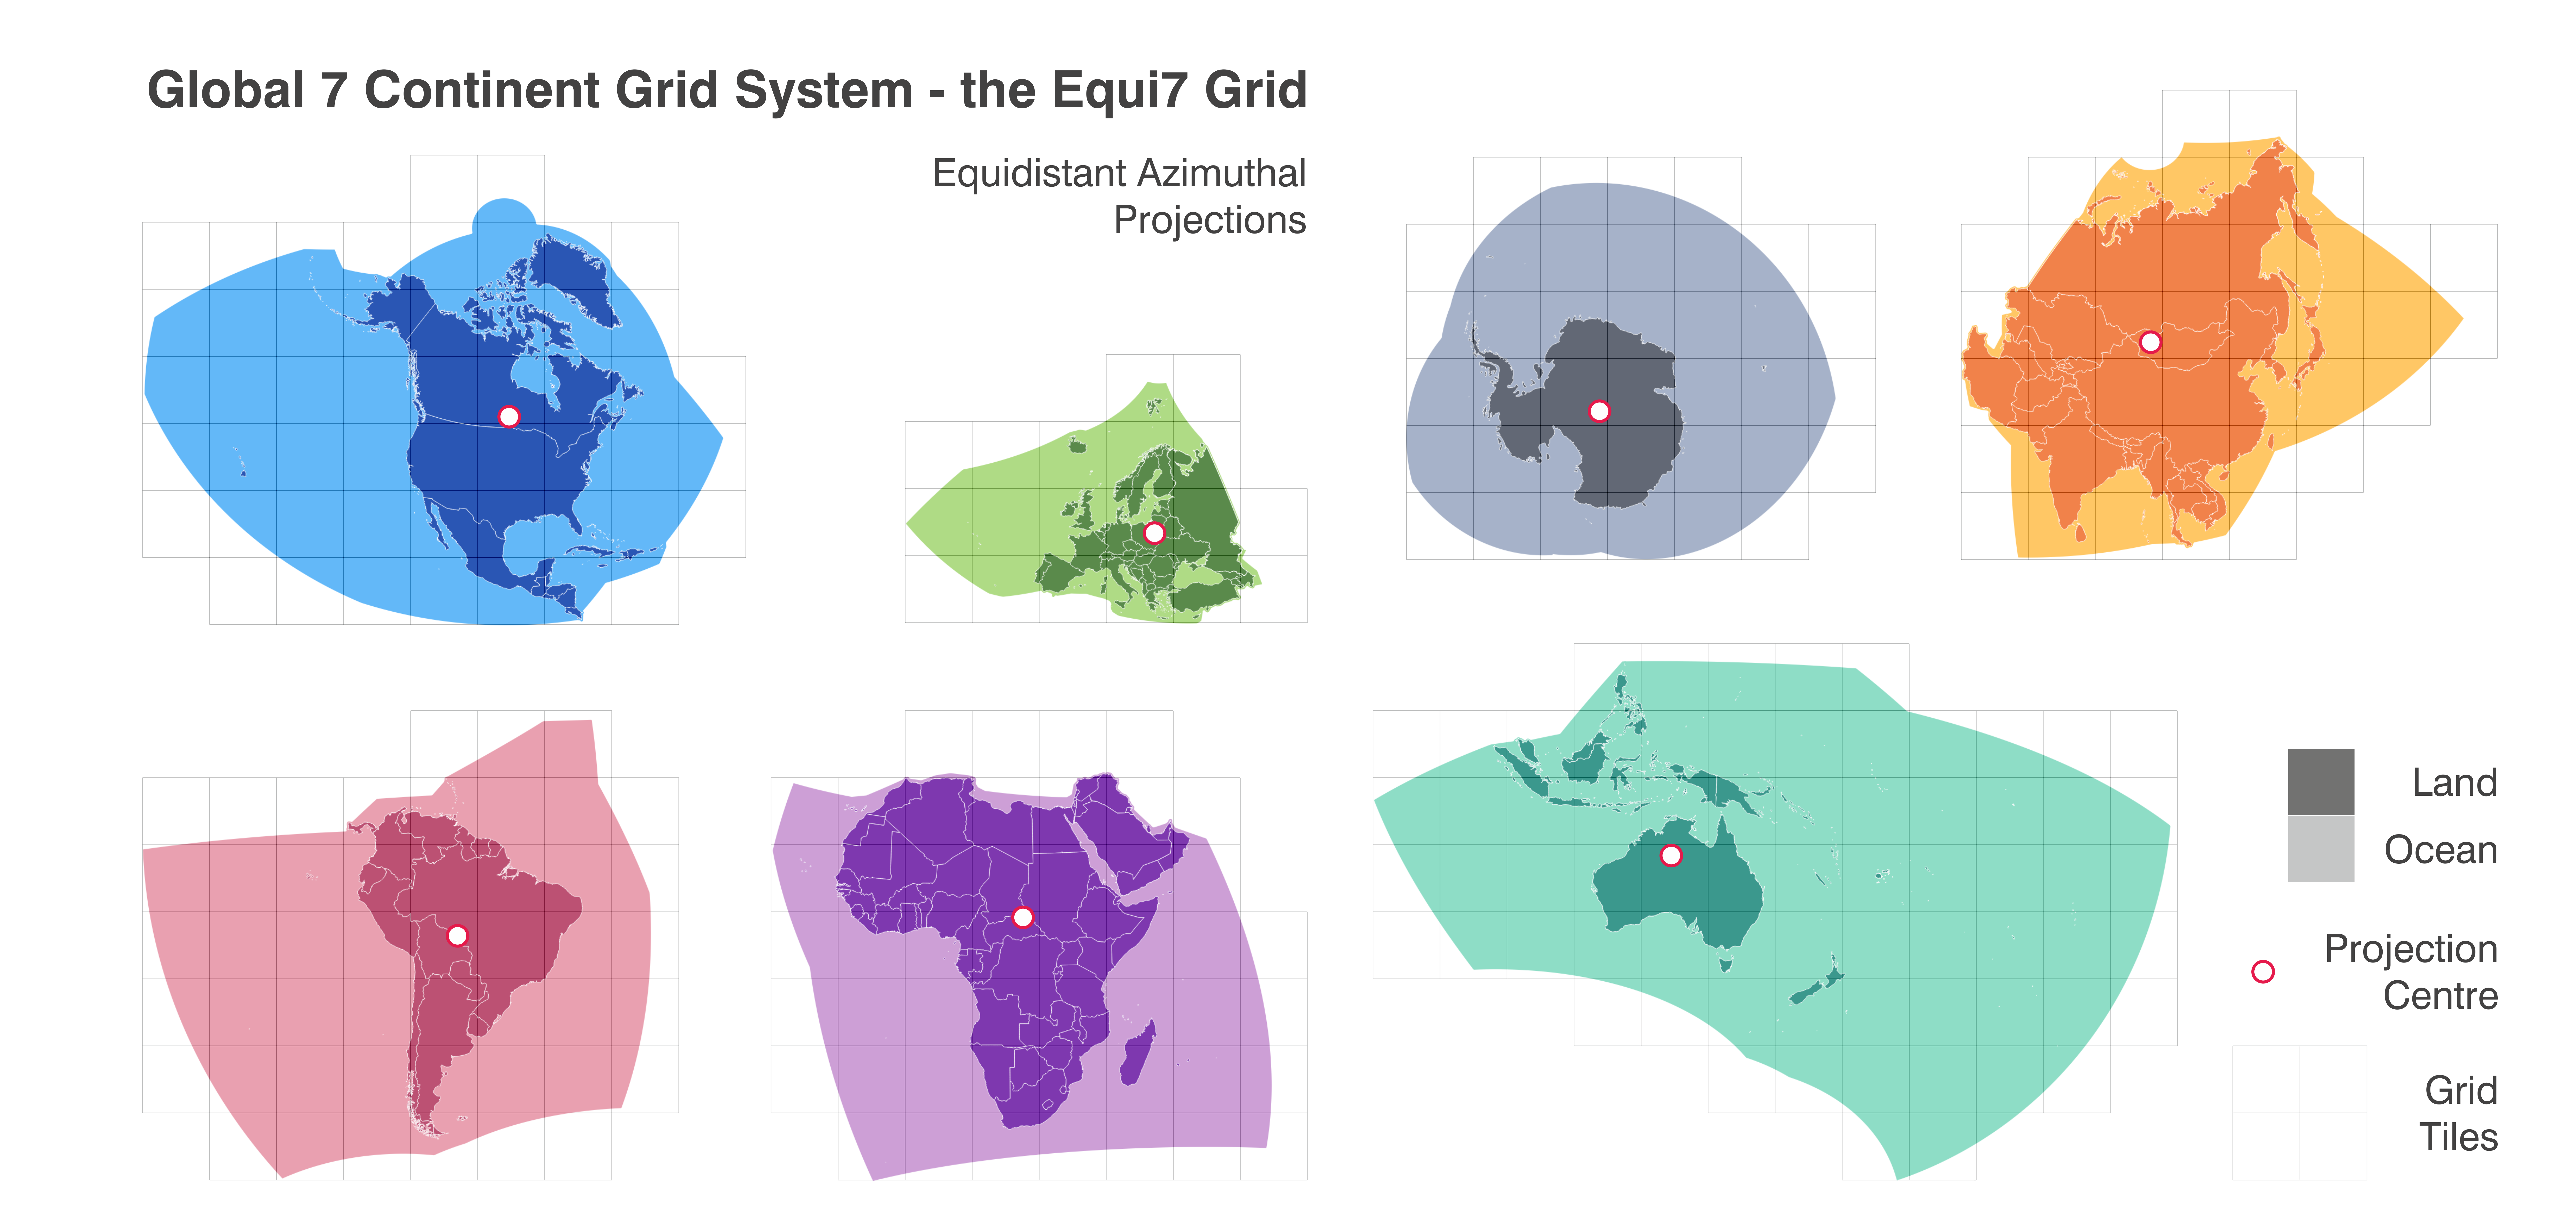
\includegraphics[width=1.0\textwidth]{7continents_grid_v11}
\caption{
The Equi7 Grid: Schematic images of the (already projected) continental zones with grid tiles and projection centres.
}
\label{fig:7cont}
\end{figure}

\section{Design and Geometry}
\label{sec:design}

\subsection{Datum}
As spatial reference the WGS84-ellipsoid (World Geodetic System 1984) was chosen for the ellipsoidal coordinates on the Earth's surface. These are necessary for the addressing of locations in the global perspective, e.g. during the assignment of satellite scenes to the subgrids. Here the ellipsoid's metrics:

\begin{table}[hbtp]
\caption[Map Projections]{
The WGS84 Ellipsoid parameters
}
\centering
	{
	\begin{tabular}{ll}
	\hline 
	Major Axis \textbf{a} & $6378137 m$ \\
	Flattening \textbf{f} & $298.257223563^{-1}$ \\
	Prime Meridian & $0.0^{\circ}$ \\
	Unit & $0.0174532925199433^{\circ}$ \\
	\hline 
	\end{tabular} 
	}
\label{tab:wgs84}
\end{table}

\subsection{Zones}
The Equi7 Grid is a regular grid which defines each location implicitly with a fixed sampling distance relative to a set of linear axis; here two orthogonal ones. As opposed to a single grid for the whole globe, Equi7 separates the globe into seven subgrids (zones) of identical type of projection. Reducing the extent of a projected grid (in respect to the Earth curvature) reduces negative effects from geometric distortions, like data oversampling or disordered pixel neighbour relationships.

Considering findings of the study of \citep{Bauer-Marschallinger2014}, and with TU-Wien's processor- and user requirements in mind, the zone borders were optimised by following requirements: 
\begin{enumerate}
\item Landmasses should form compact entities
\item Borders should be preferably over oceans
\item Countries should preferably be not split
\end{enumerate}

The seven grids cover the Earth entirely without gap and with 50km overlap over land borders. A global overview of the delineation is shown in Figure \ref{fig:gridzones}.

\begin{figure}[hbtp]
\centering
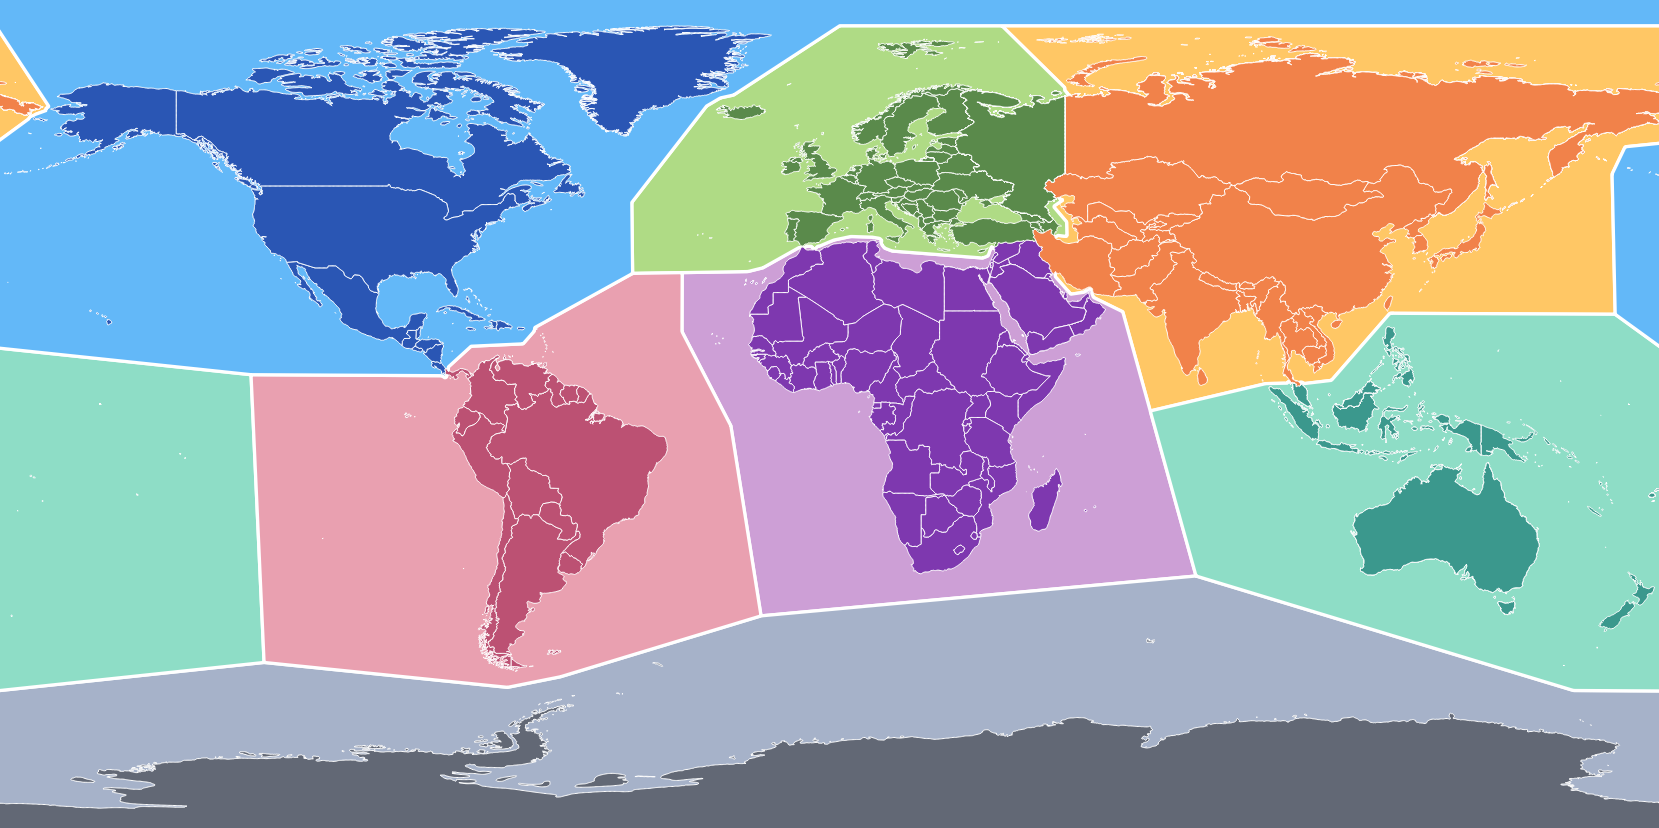
\includegraphics[width=1.0\textwidth]{equi7_grid_v11_overview}
\caption{
Continental zone partitioning into the seven subgrids, projected for global overview to the Plate Carr\'{e}e (aka geographic aka Lat-Lon, using WGS84 coordinates).
}
\label{fig:gridzones}
\end{figure}

The zones are defined by manually created shapefiles following above rules 1-3 in the WGS84 space. After transformation to the individual projections (see Section \ref{sub:projections}), zone borders over land are buffered to a 50km extent to allow correct spatial filter operations also on the zone limits. Table \ref{tab:zones} lists the zones' basic facts. 

\begin{table}[hbtp]
\caption[Zone Facts]{
The Equi7 Grid zones.
}
\centering
	{
	\begin{tabular}{lccr}
	\textbf{Zone} & \textbf{Short Name} & \textbf{Colour} & \textbf{Covered Land Area} \\
	& & & [Mio. km$^{2}$] \\
	\hline
	North America & NA & blue & 24.2 \\
	Europe & EU & green & 9.7 \\
	Asia & AS & orange & 38.6 \\
	South America & SA & red & 17.9 \\
	Africa & AF & purple & 33.6 \\
	Oceania & OC & turquoise & 11.2 \\
	Antarctica & AN & gray & 12.3 \\
	\hline
	\end{tabular} 
	}
\label{tab:zones}
\end{table}

\newpage

\subsection{Projections}
\label{sub:projections}

All seven zone are projected from ellipsoidal coordinates (lat/lon) in WGS84 to planar grids using the \textit{Equidistant Azimuthal Projection}. Figure \ref{fig:equi_azi} exemplifies the projection in oblique aspects. 

\subsubsection{The Azimuthal Equidistant}

\begin{figure}[hbtp]
\centering
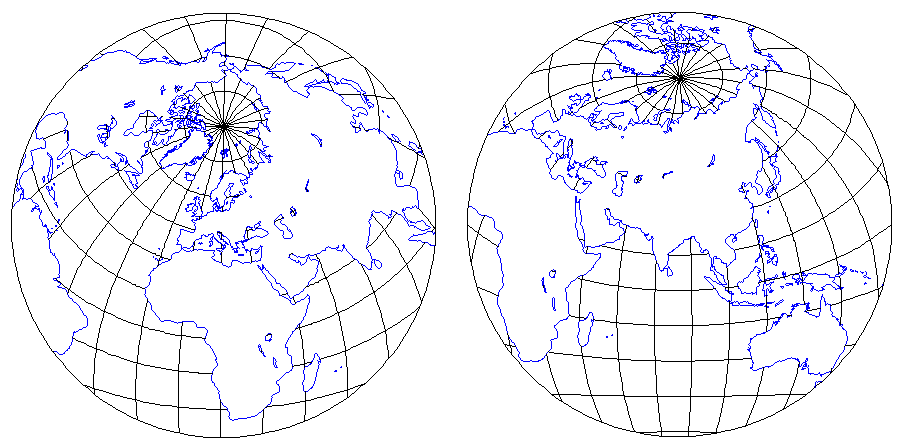
\includegraphics[width=0.9\textwidth]{equi_azi}
\caption{
The Azimuthal Equidistant Projection in oblique aspect centred over Austria (left) and Nepal (right). Linear scales emanating from the projection centre are undistorted. Distortion of angles and areas increases with distance to the centre.
}
\label{fig:equi_azi}
\end{figure}

The calculation of the planar coordinates $x$ and $y$ (the \textit{forward projection}) implies the solving of the \textit{inverse geodesic problem}, that is

\begin{eqnarray}
dx &=& c \sin Az \\ 
dy &=& c \cos Az \\
x &=& dx + FE \\
y &=& dy + FN
\end{eqnarray}

where $x$ and $y$ the are location's Easting and Northing, $c$ is the length and \textit{Az} is the azimuth from north of the geodesic line between the location and the projection centre ($\phi_{0}$, $\lambda_{0}$), $FE$ the false Easting, and $FN$ the false Northing. The \textit{inverse projection} from planar to ellipsoidal coordinates (geodetic latitude $\phi$ and longitude $\lambda$) depicts the \textit{direct geodetic problem} and starts with the determination of \textit{Az} and $c$:

\begin{eqnarray}
dx &=& x - FE \\
dy &=& y - FN \\
\mathit{Az} &=& \arctan \dfrac{dy}{dx} \\
c &=& \sqrt{dx^2 + dy^2}
\end{eqnarray}

Both, the forward and inverse projection of the ellipsoid involve the solving of elliptic integrals that are favourably computed with numerical methods. \cite{Snyder1987} gives approximating formulae and general information on the projection. However, these formulae lead to significant geometric inaccuracies in areas far from the projection centre. Thus, a more recent approach following findings of \citep{Karney2011, Karney2013} is selected for the transformation between geographical and projected coordinates (degrees and metres; see Section \ref{sub:proj_impl}).

\subsubsection{Equi7 Projections}

The parameters of the Azimuthal Equidistant have been individually optimised in means of minimising data oversampling estimated by the mean \textit{grid oversampling factor} as described in \cite{Bauer-Marschallinger2014}. The optimised parameters for each zone are listed in Table \ref{tab:projections}. For Antarctica, the South Pole is conveniently chosen as origin, since it is almost co-located with the the optimal origin and the additional error is insignificant. False Easting and -Northing are set so that negative coordinates are avoided. 

\begin{table}[hbtp]
\caption[Projection Parameter]{
The Equi7 Grid projection parameters for the Azimuthal Equidistant. With $\lambda_{0}$ as central meridian and $\phi_{0}$ as latitude of origin.
}
\centering
	{
	\begin{tabular}{lrrrr}
	\hline
	Parameter & $\mathbf{\lambda_{0}}$ & $\mathbf{\phi_{0}}$ & False Easting & False Northing \\
	Zone / Unit & $^{\circ}E$ & $^{\circ}N$ & m & m \\
	\hline
	North America & $-111.0$ & $47.5$ & $8264722.18$ & $4867518.35$ \\
	Europe & $24.0$ & $53.0$ & $5837287.82$ & $2121415.70$ \\
	Asia & $94.0$ & $47.0$ & $4340913.85$ & $4812712.92$ \\
	South America & $-60.5$ & $-14.0$ & $7257179.24$ & $5592024.45$ \\
	Africa & $21.5$ & $8.5$ & $5621452.02$ & $5990638.42$ \\
	Oceania & $131.5$ & $-19.5$ & $6988408.54$ & $7654884.54$ \\
	Antarctica & $0.0$ & $-90.0$ & $3714266.98$ & $3402016.51$ \\
	\hline
	\end{tabular} 
	}
\label{tab:projections}
\end{table}

The individual \textit{Well-Known-Text}-strings giving the full georeference information are the following:

\subsubsection*{America}

\begin{lstlisting}
PROJCS["Azimuthal_Equidistant",GEOGCS["GCS_WGS_1984",DATUM["D_WGS_1984",SPHEROID["WGS_1984",6378137.0,298.257223563]],PRIMEM["Greenwich",0.0],UNIT["Degree",0.0174532925199433]],PROJECTION["Azimuthal_Equidistant"],PARAMETER["false_easting",8264722.17686],PARAMETER["false_northing",4867518.35323],PARAMETER["central_meridian",-97.5],PARAMETER["latitude_of_origin",52.0],UNIT["Meter",1.0]]
\end{lstlisting}

\subsubsection*{Europe}

\begin{lstlisting}
PROJCS["Azimuthal_Equidistant",GEOGCS["GCS_WGS_1984",DATUM["D_WGS_1984",SPHEROID["WGS_1984",6378137.0,298.257223563]],PRIMEM["Greenwich",0.0],UNIT["Degree",0.0174532925199433]],PROJECTION["Azimuthal_Equidistant"],PARAMETER["false_easting",5837287.81977],PARAMETER["false_northing",2121415.69617],PARAMETER["central_meridian",24.0],PARAMETER["latitude_of_origin",53.0],UNIT["Meter",1.0]]
\end{lstlisting}

\subsubsection*{Asia}

\begin{lstlisting}
PROJCS["Azimuthal_Equidistant",GEOGCS["GCS_WGS_1984",DATUM["D_WGS_1984",SPHEROID["WGS_1984",6378137.0,298.257223563]],PRIMEM["Greenwich",0.0],UNIT["Degree",0.0174532925199433]],PROJECTION["Azimuthal_Equidistant"],PARAMETER["false_easting",4340913.84808],PARAMETER["false_northing",4812712.92347],PARAMETER["central_meridian",94.0],PARAMETER["latitude_of_origin",47.0],UNIT["Meter",1.0]]
\end{lstlisting}

\subsubsection*{South America}

\begin{lstlisting}
PROJCS["Azimuthal_Equidistant",GEOGCS["GCS_WGS_1984",DATUM["D_WGS_1984",SPHEROID["WGS_1984",6378137.0,298.257223563]],PRIMEM["Greenwich",0.0],UNIT["Degree",0.0174532925199433]],PROJECTION["Azimuthal_Equidistant"],PARAMETER["false_easting",7257179.23559],PARAMETER["false_northing",5592024.44605],PARAMETER["central_meridian",-60.5],PARAMETER["latitude_of_origin",-14.0],UNIT["Meter",1.0]]
\end{lstlisting}

\newpage

\subsubsection*{Africa}

\begin{lstlisting}
PROJCS["Azimuthal_Equidistant",GEOGCS["GCS_WGS_1984",DATUM["D_WGS_1984",SPHEROID["WGS_1984",6378137.0,298.257223563]],PRIMEM["Greenwich",0.0],UNIT["Degree",0.0174532925199433]],PROJECTION["Azimuthal_Equidistant"],PARAMETER["false_easting",5621452.01998],PARAMETER["false_northing",5990638.42298],PARAMETER["central_meridian",21.5],PARAMETER["latitude_of_origin",8.5],UNIT["Meter",1.0]]
\end{lstlisting}

\subsubsection*{Oceania}

\begin{lstlisting}
PROJCS["Azimuthal_Equidistant",GEOGCS["GCS_WGS_1984",DATUM["D_WGS_1984",SPHEROID["WGS_1984",6378137.0,298.257223563]],PRIMEM["Greenwich",0.0],UNIT["Degree",0.0174532925199433]],PROJECTION["Azimuthal_Equidistant"],PARAMETER["false_easting",5621452.01998],PARAMETER["false_northing",5990638.42298],PARAMETER["central_meridian",21.5],PARAMETER["latitude_of_origin",8.5],UNIT["Meter",1.0]]
\end{lstlisting}

\subsubsection*{Antarctica}

\begin{lstlisting}
PROJCS["Azimuthal_Equidistant",GEOGCS["GCS_WGS_1984",DATUM["D_WGS_1984",SPHEROID["WGS_1984",6378137.0,298.257223563]],PRIMEM["Greenwich",0.0],UNIT["Degree",0.0174532925199433]],PROJECTION["Azimuthal_Equidistant"],PARAMETER["false_easting",3714266.97719],PARAMETER["false_northing",3402016.50625],PARAMETER["central_meridian",0.0],PARAMETER["latitude_of_origin",-90.0],UNIT["Meter",1.0]]
\end{lstlisting}

\newpage

\subsection{Tiling}

The seven planar grid zones are independently divided into square tiles. Point of reference is \textit{LowerLeft} -- for the tile numbering as well as for the grid coordinates. Figure \ref{fig:tiling} explains the principles of the tiling system, whereas Figure \ref{fig:tiling_africa} illustrates them on the example of the Africa grid. Please note the projection centre that coincide with the centre of land area (indicated as white dot). 

Tiles are defined in squares that are (partially) overlapping with the grid zone. Consequently, there are sections of tiles that are not defined by the individual grid zone but are actually covering area that is in realm of the neighbouring continent grid zone (bright orange areas in Fig. \ref{fig:tiling_africa}).

\begin{figure}[hbtp]
\centering
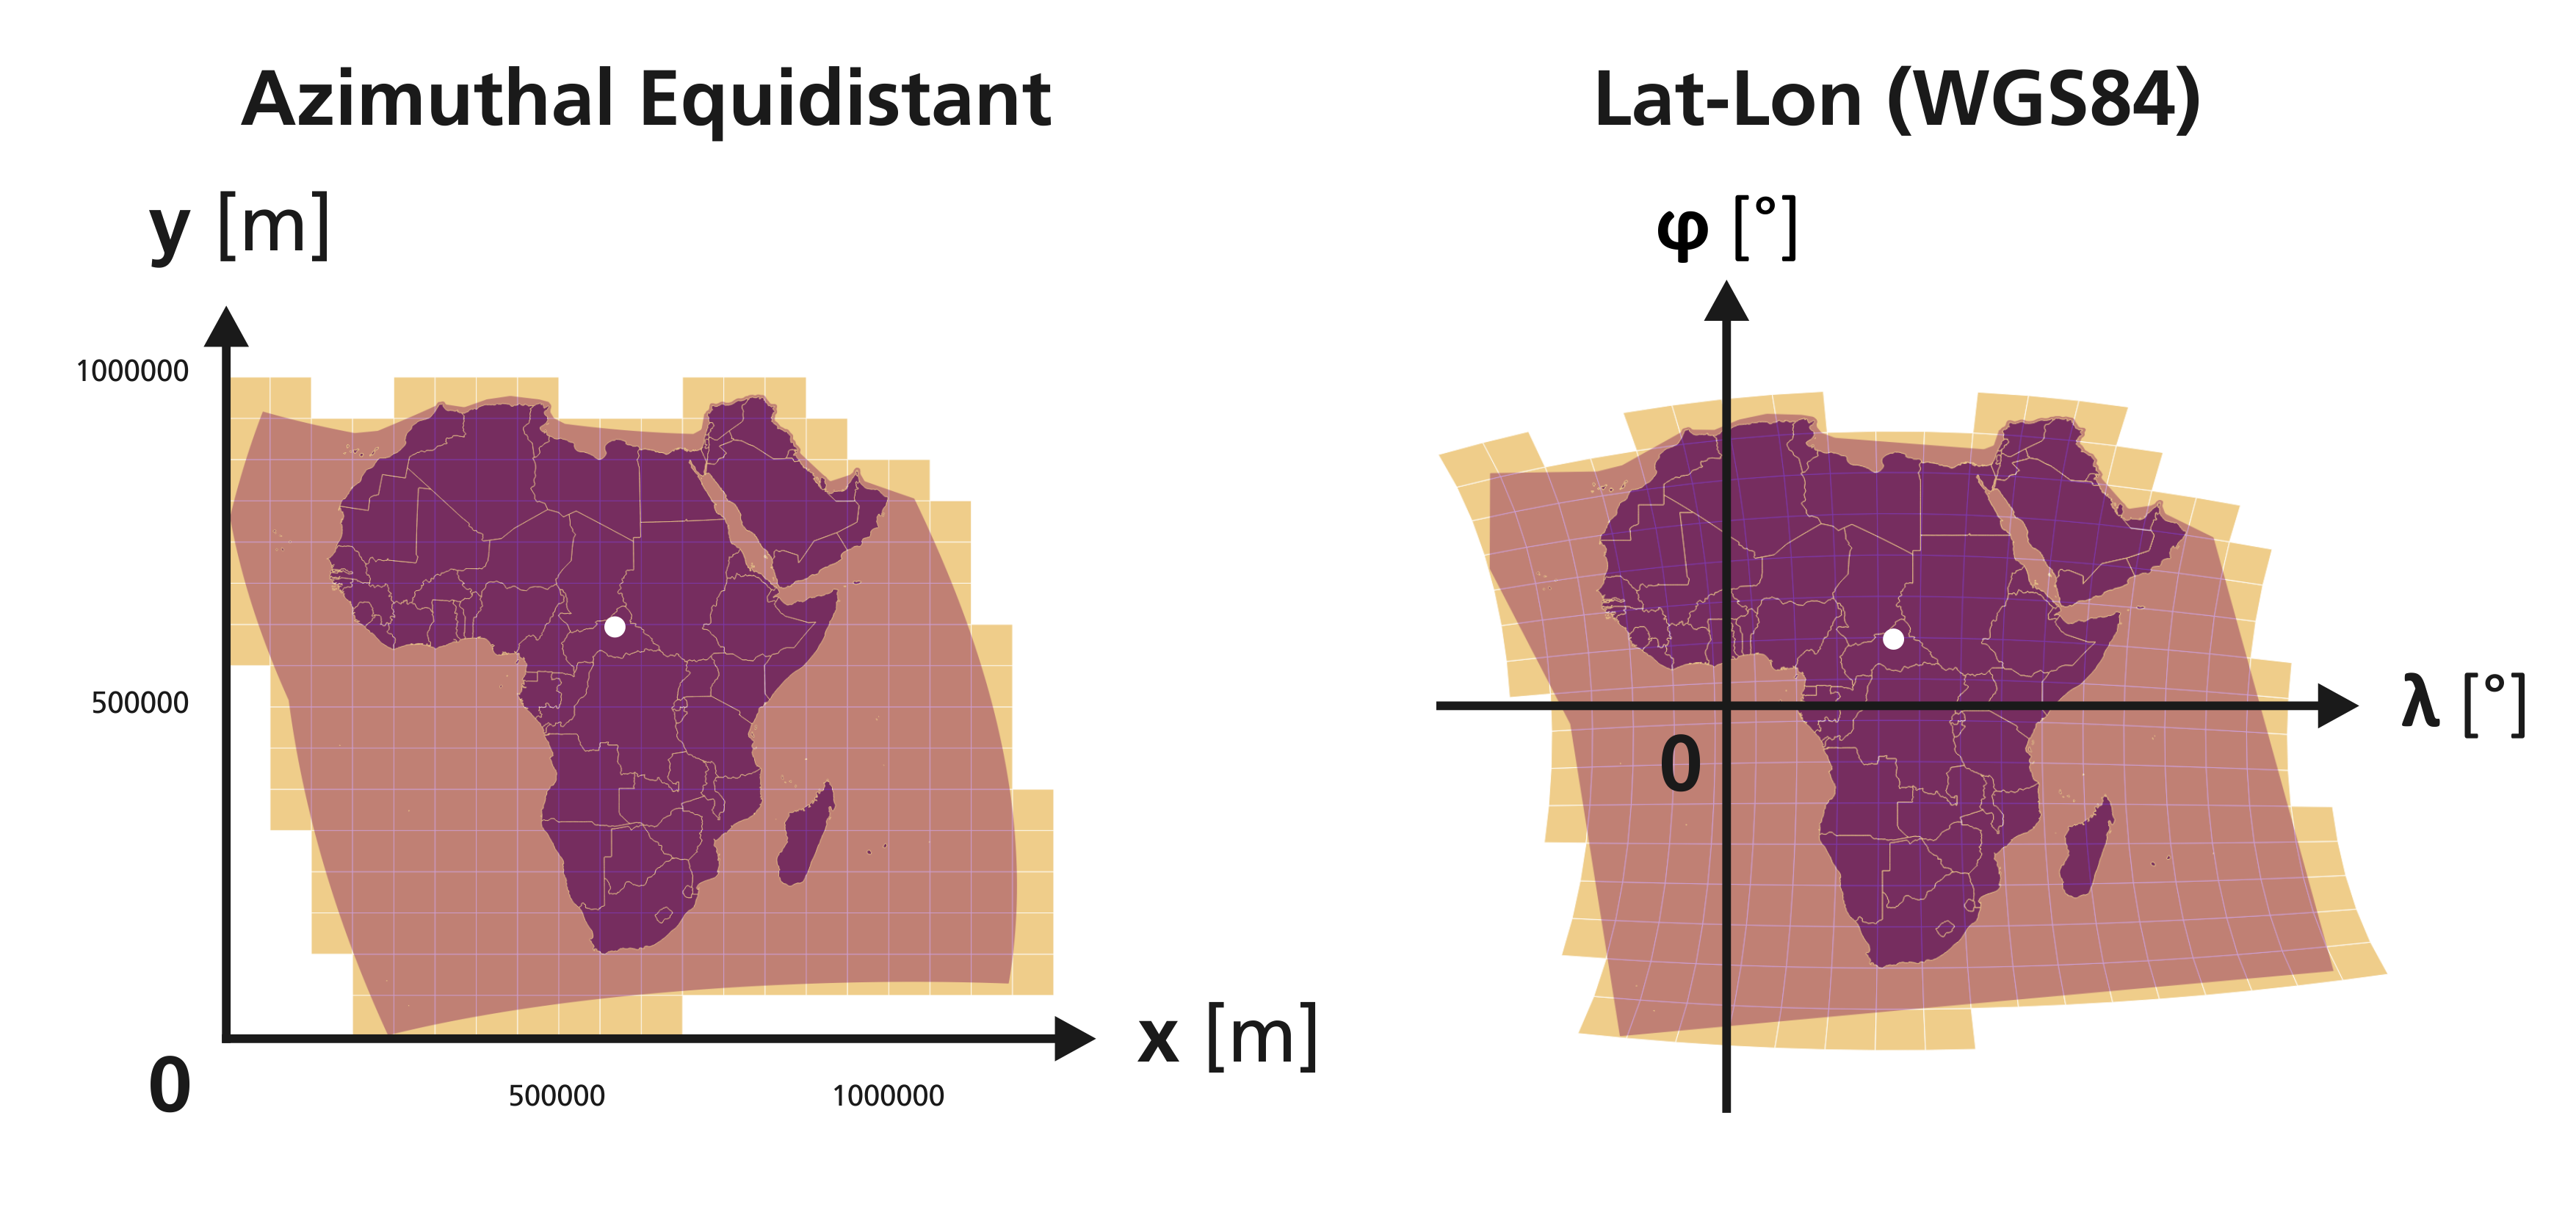
\includegraphics[width=0.9\textwidth]{equi7_tiling_africa}
\caption{
Realisation of the Equi7 grid tiling on the example of the African grid, displayed in the Equi7- and geographic space. Please note the different shapes of the tiles and boundaries. The white dot indicates the centre of origin of the Azimuthal Equidistant projection.
}
\label{fig:tiling_africa}
\end{figure}

\subsubsection*{Tiling Levels}

The Equi7 Grid V13 features multiple levels of tilings, meeting the different requirements during processing images of low and high spatial resolution and data volumes. By reducing the tile extent, the number of pixels per tiled image remains operable even at high resolutions. This setup ensures also that the different levels are mutually aligning and congruent. 

In version 13, three levels have been chosen for low, medium and high resolution spatial data. Table \ref{tab:tilelevels} lists basic characteristics of these tiling levels \textbf{T6}, \textbf{T3}, and \textbf{T1}:

\begin{table}[hbtp]
\caption[Tile Levels]{
The Equi7 Grid Tiling Levels for different target samplings.
}
\centering
	{
	\begin{tabular}{lccc}
	\hline 
	Tiling Level Code & \textbf{T6} & \textbf{T3} & \textbf{T1} \\ 
	Tile Extents & 600km & 300km & 100km \\
	Typical Pixel Sampling & 500m / 75m & 40m & 10m / 5m \\ 
	Samples (1 Axis) & 1200 / 8000 & 7500 & 10000 / 20000 \\ 
	\hline 
	\end{tabular}	
	}
\label{tab:tilelevels}
\end{table}




\begin{figure}[hbtp]
\centering
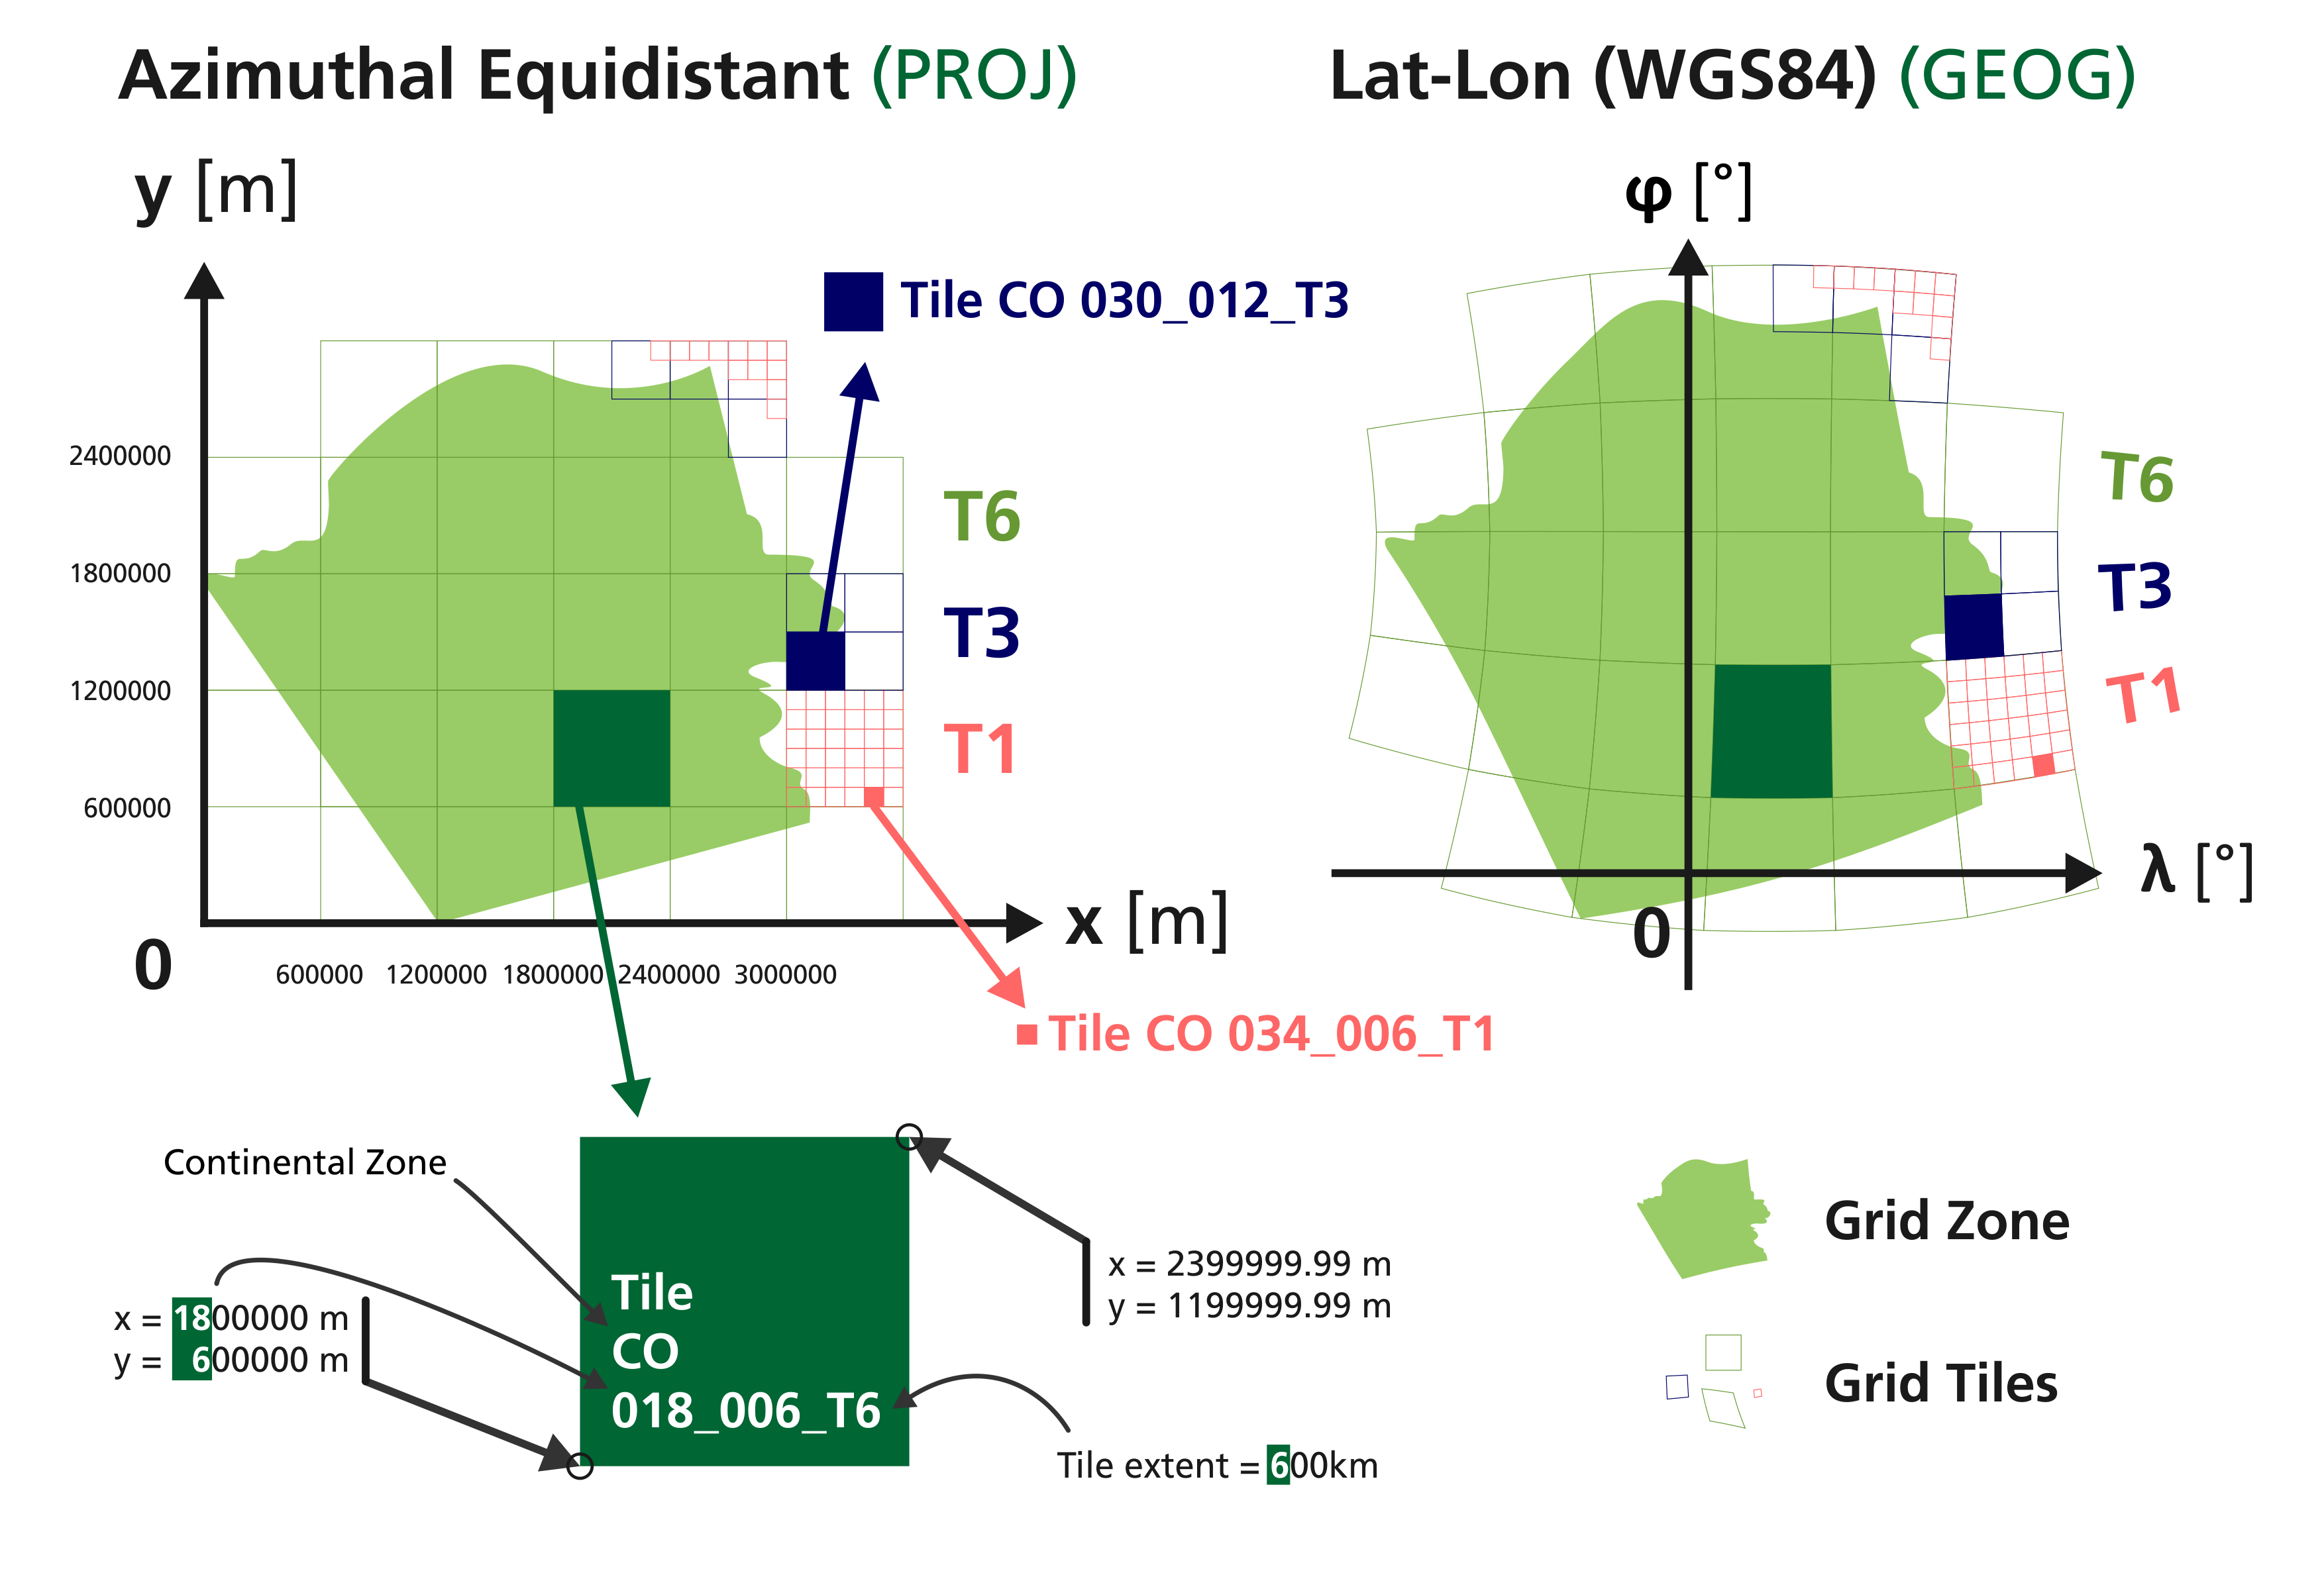
\includegraphics[width=0.9\textwidth]{equi7_v13_tiling}
\caption{
Schematic relationship of the Equi7 subgrids (left, folder name PROJ) and the geographic Lat-Lon coordinate system (right, folder name GEOG). With exemplary tile namings in green, blue and orange for T6, T3, and T1 tile layer, respectively. \textsl{CO} is a placeholder for the grid continent's acronym as in Tab. \ref{tab:zones}.
}
\label{fig:tiling}
\end{figure}

\subsubsection*{Shapefile Tile Naming}



As evident from Fig. \ref{fig:tiling}, the tiles are not ordinary numbered but named after the coordinates of the lower left corner:

\texttt{\textbf{Unique Tilename = E7G co eee\_nnn\ Tt}} \\
\\
\texttt{E7G = Equi7 Grid} \\
\texttt{co = continental zone acronym} \\
\texttt{eee = Easting lower left corner} \\
\texttt{nnn = Northing lower left corner} \\
\texttt{Tt = tile extent}


And as example:

\texttt{Tilename = E7G AF 018\_006 T6}


\subsubsection*{Tiling Statistics}

When it comes to the design of data processing engines, the number of tiles and furthermore the number of tiles covering land surfaces are of special interest. Table \ref{tab:tilestatistics} summarises these statistics.

% Table generated by Excel2LaTeX from sheet 'Sheet1'
\begin{table}[htbp]
  \centering
  \caption{Statistics of Tiling Levels in comparison to Earth's surface area as from Wikipedia. Displaying, per Tiling Level, the number of total tiles, tiles over land and the total area of all tiles and corresponding ratios.}
    \begin{tabular}{lrrr}
    \hline
     & \textit{Area Total} & \textit{Area Land} & \% Land \\
    \textbf{Wikipedia} - Earth surface area [$km^{2}$] & 510072000 & 148940000 & \textit{\textbf{29\%}} \\
    \\
    \hline
    \textit{Zone} & \textit{Tiles Total} & \textit{Tiles Land} & \textit{\% Land} \\
	\hline
	\\    
    \textit{\textbf{Tiling Level T6}} \\
    AF    & 266   & 147   & 55\% \\
    AN    & 213   & 68    & 32\% \\
    AS    & 228   & 168   & 74\% \\
    EU    & 94    & 61    & 65\% \\
    NA    & 286   & 132   & 46\% \\
    OC    & 429   & 170   & 40\% \\
    SA    & 273   & 86    & 32\% \\
    \hline
    \textit{\textbf{WORLD}} & \textit{\textbf{1789}} & \textit{\textbf{832}} & \textit{\textbf{47\%}} \\
    \hline
    Total Tile Area [$km^{2}$] & 644040000 & 299520000 &  \\
    Ratio to Area from Wikipedia & 126\% & 201\% &  \\
    \hline
    \\    
    \textit{\textbf{Tiling Level T3}} \\
    AF    & 1004  & 487   & 49\% \\
    AN    & 792   & 211   & 27\% \\
    AS    & 829   & 592   & 71\% \\
    EU    & 340   & 196   & 58\% \\
    NA    & 1065  & 438   & 41\% \\
    OC    & 1611  & 397   & 25\% \\
    SA    & 1009  & 273   & 27\% \\
    \hline
    \textit{\textbf{WORLD}} & \textit{\textbf{6650}} & \textit{\textbf{2594}} & \textit{\textbf{39\%}} \\
    \hline
    Total Tile Area [$km^{2}$] & 598500000 & 233460000 &  \\
    Ratio to Area from Wikipedia & 117\% & 157\% &  \\
    \hline
    \\   
    \textit{\textbf{Tiling Level T1}} \\
    AF    & 8603  & 3788  & 44\% \\
    AN    & 6793  & 1504  & 22\% \\
    AS    & 7089  & 4504  & 64\% \\
    EU    & 2823  & 1341  & 48\% \\
    NA    & 9185  & 3149  & 34\% \\
    OC    & 13830 & 1966  & 14\% \\
    SA    & 8645  & 2051  & 24\% \\
    \hline
    \textit{\textbf{WORLD}} & \textit{\textbf{56968}} & \textit{\textbf{18303}} & \textit{\textbf{32\%}} \\
    \hline
    Total Tile Area [$km^{2}$] & 569680000 & 183030000 &  \\
    Ratio to Area from Wikipedia & 112\% & 123\% &  \\
	\hline
    \end{tabular}%
  \label{tab:tilestatistics}%
\end{table}%

\newpage

\section{Production and Structure}
\label{sec:production}

\subsection{Projection Implementation}
\label{sub:proj_impl}

At TU Wien, the Equi7-projections are computed with a python software on a Linux system, using \textit{PROJ.4} via \textit{GDAL/OGR}.

The Equi7 uses a precise algorithm including iterations, as described in \cite{Karney2013}, yielding effectively following equation for inverse and direct geodetic problem, here in the python-notation of the \textit{GeographicLib} library:

\begin{eqnarray}
\left[ c, \mathit{Az} \right] &=& \mathrm{Geodesic.WGS84.Inverse}(\phi_{0}, \lambda_{0}, \phi, \lambda) \\
\left[ \phi , \lambda \right] &=& \mathrm{Geodesic.WGS84.Direct}(\phi_{0}, \lambda_{0}, \mathit{Az}, c)
\end{eqnarray}

Above formulae (including formulae from Section \ref{sub:projections}) are implemented in a modified version of the \textit{proj-4.8.0} library, replacing the approximating formulae of \citep{Snyder1987} in the source code file

\texttt{PJ\_aeqd.c}. 

Those are called via \textit{GDAL/OGR 1.10.0}. The enhancements were reported to the proj.4 project so that it will be included in upcoming releases. In the meantime (Equi7 V12, November 2014), a batch for Linux systems, 

\texttt{proj-4.8.0\_tu\_wien\_batch.zip},

is set up to apply all necessary changes to the official release of proj.4. As a note, the resulting Equi7 shapefiles and DEMs are practically identical to results produced with \textit{ArcGIS 10.2} via its Python module \textit{arcpy}.

\newpage

\subsection{Grid Defining Files}
\label{definingfiles}

The Equi7 Grid Version 13 constitutes of four main components:

\begin{itemize}[itemsep=0.1ex]
\item Shapefiles
\begin{itemize}
\item Geometries
\end{itemize}
\item DEM Geotiffs
\begin{itemize}
\item 7 Zone DEMs
\item DEM Tiles
\end{itemize}
\item Code and Seedfiles
\begin{itemize}
\item Generating code
\item Seed shapefiles for zone and country boundaries in WGS84
\item Projection files
\end{itemize}
\item Documentation
\end{itemize}

Figure \ref{fig:equi7_v13_file_structure} displays the file structure and lists all elements of the Equi7 Grid. There are five types of datasets:

\paragraph{Zone Shapefile}
\texttt{EQUI7\_V13\_co\_PROJ\_ZONE.shp}

A (vector-) shapefile determining the outline of the continental subgrids. \texttt{co} holds place for the continent name. \texttt{proj} for the coordinate space.

\paragraph{Tiles Shapefile}
\texttt{EQUI7\_V13\_co\_PROJ\_TILE\_Tt.shp}

A (vector-) shapefile carrying the outline of the zone's tiles.

\paragraph{Land Shapefile}
\texttt{EQUI7\_V13\_co\_PROJ\_LAND.shp}

A (vector-) shapefile describing the country borders as provided by the \textit{TM\_WORLD\_ BORDERS-0.3}.

\paragraph{Zone DEM File}
\texttt{EQUI7\_V13\_GT30S\_co\_rrrM\_NOTTILED.tif}

A geotiff carrying the GTOPO30SRTM DEM for the entire continental zone as one piece. In combination with the letter \texttt{M}, \texttt{rrr} holds place for the sampling in metres; with \texttt{K}, in kilometres.

\paragraph{Tile DEM File}
\texttt{EQUI7\_V13\_GT30S\_co\_rrrM\_EeeeNnnn.tif}

A geotiff carrying the GTOPO30SRTM DEM for the individual tile. \texttt{co} holds place for the continent acronym; \texttt{eee} for the Easting of the lower left pixel; and \texttt{nnn} for the Northing; in 10000 metres. In combination with the letter \texttt{M}, \texttt{rrr} holds place for the sampling in metres; with \texttt{K}, in kilometres.

\begin{figure}
\centering
\noindent\makebox[\textwidth]{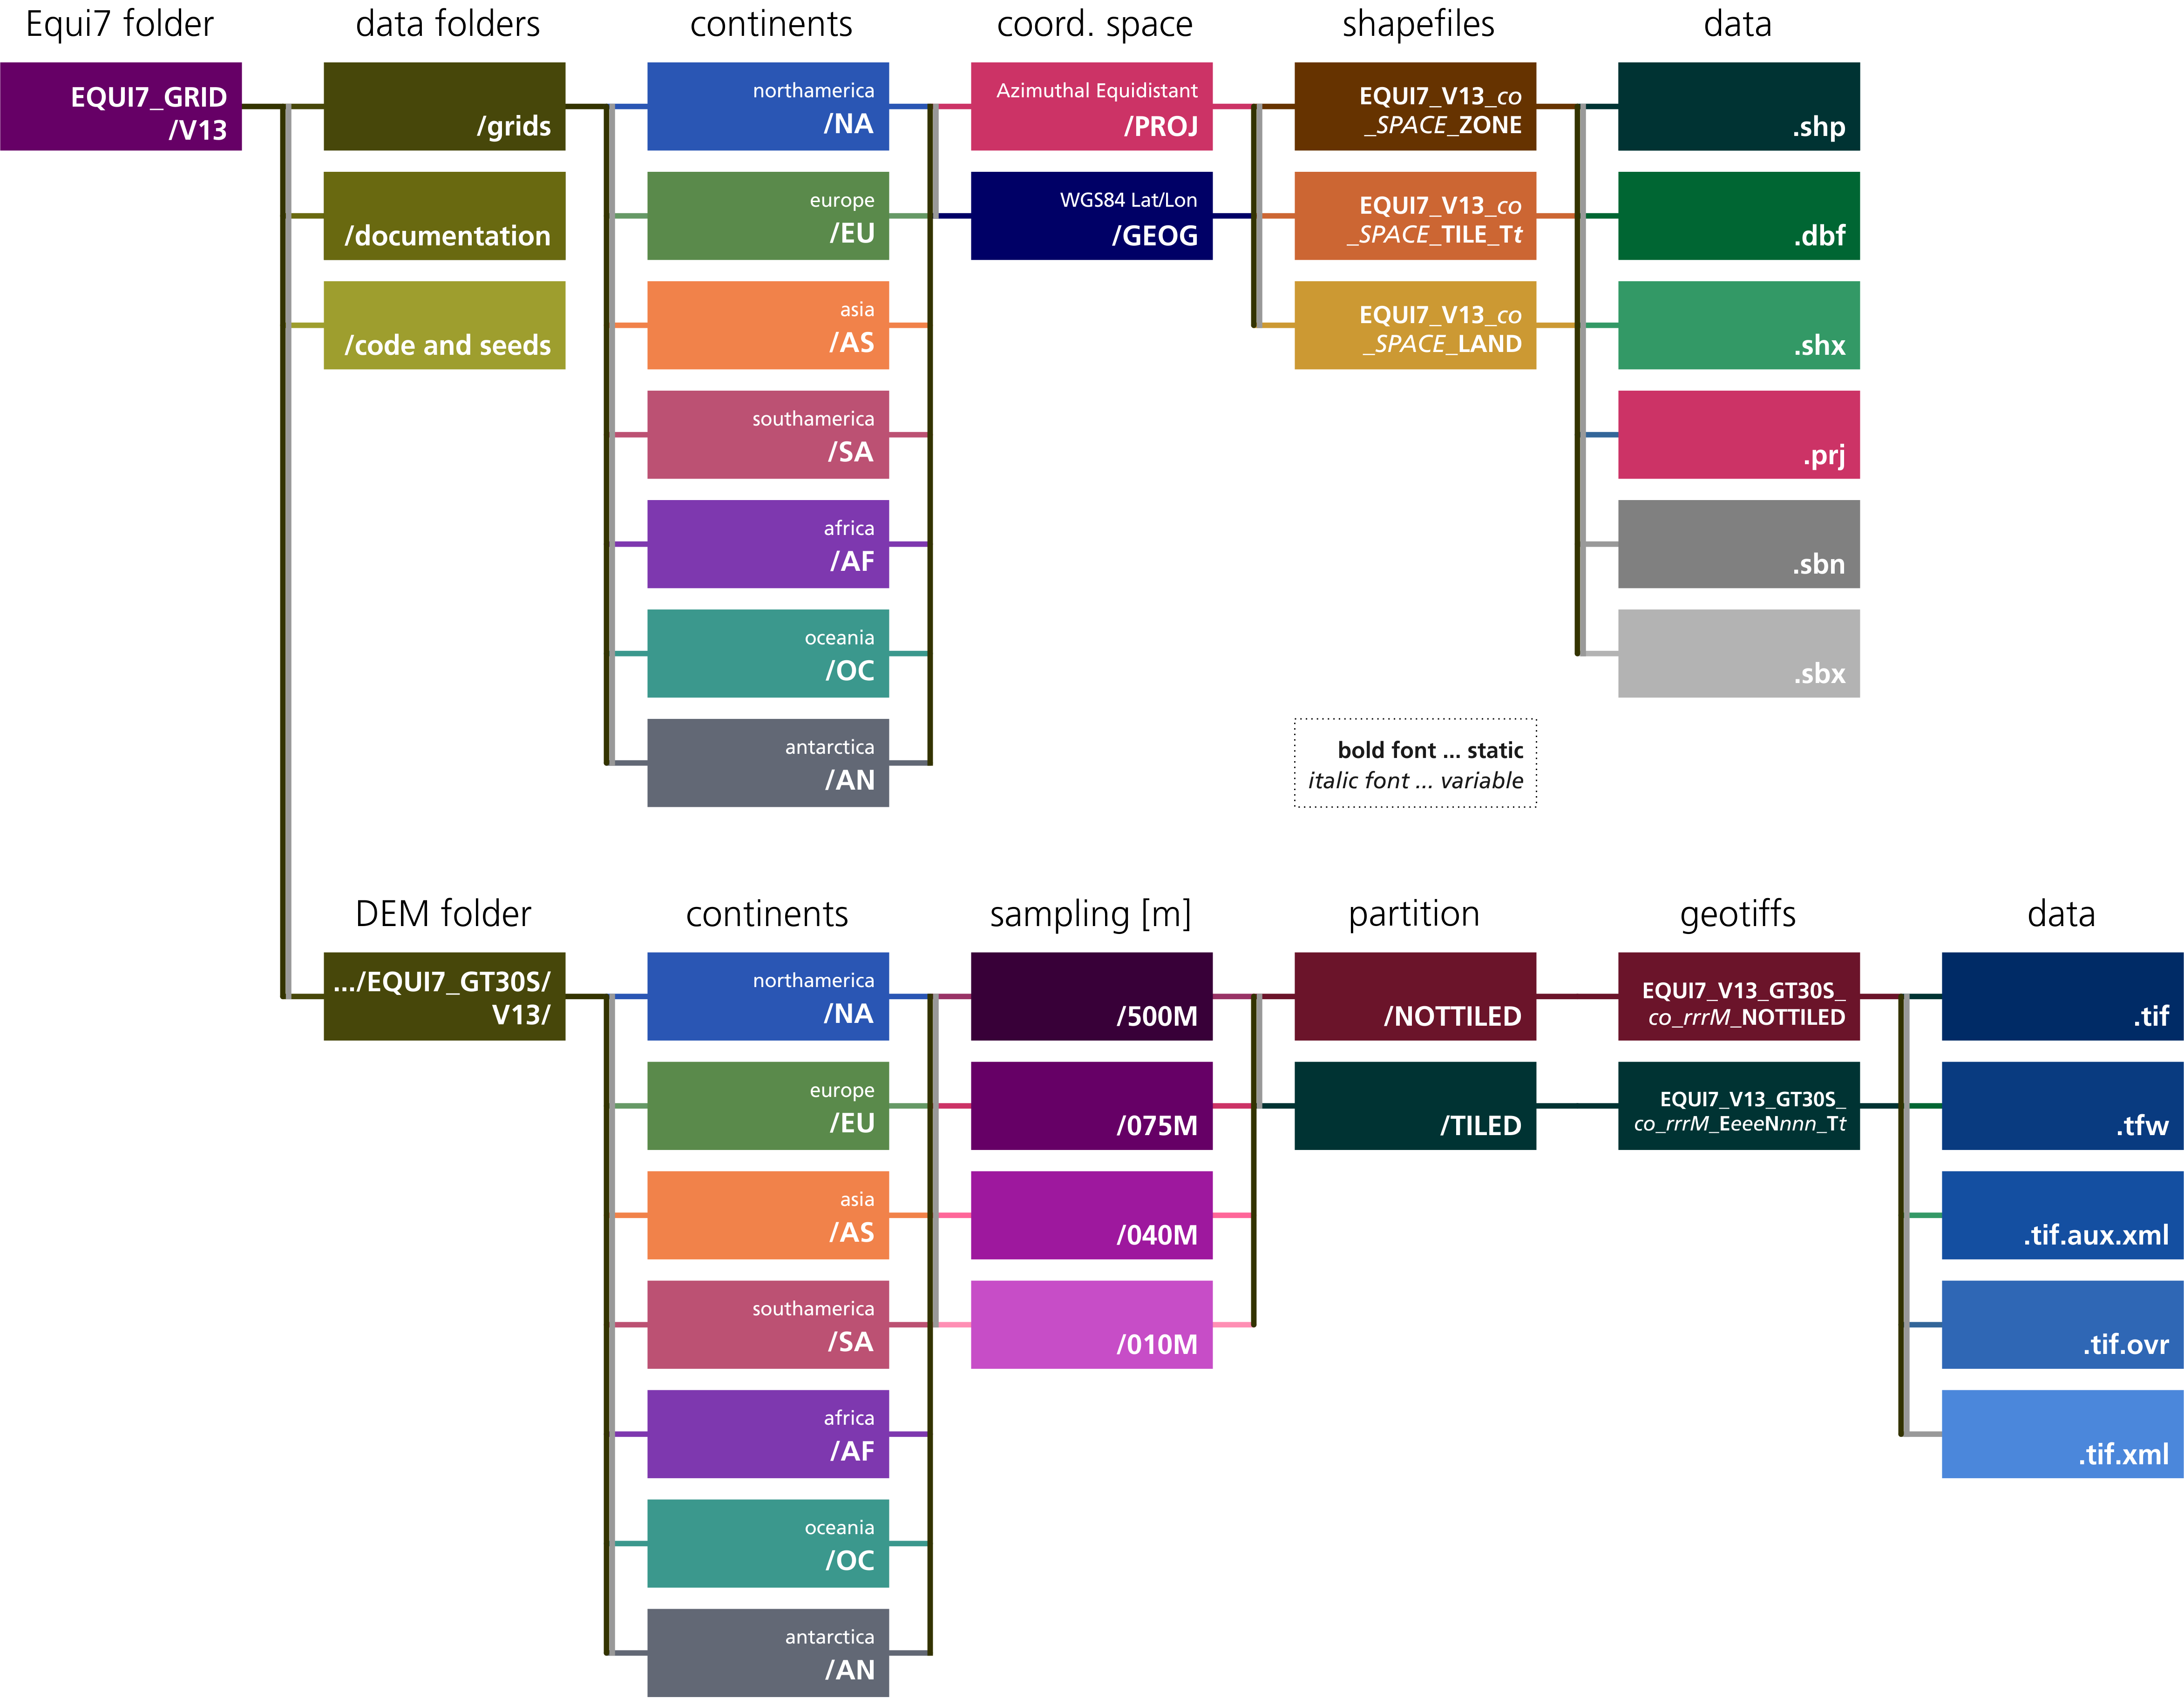
\includegraphics[width=1.3\textwidth]{equi7_v13_file_structure}}
\caption{
File structure of the Equi7 Grid Version 13. Documentation and code- and seed-files are not displayed. \textsf{co} is a placeholder for the continent's name; \textsf{SPACE} for the coordinate space (\textsf{PROJ} = Azimuthal Equidistant; \textsf{GEOG} = geographic/ellipsoidal); \textsf{rrrM} for the sampling in metres; \textsf{rrrK} for the sampling in kilometres; \textsf{eee} for the Easting; \textsf{nnn} the Northing in 10 kilometres; \textsf{t} for the tile extent in 100 kilometres.
}
\label{fig:equi7_v13_file_structure}
\end{figure}

\newpage

\section{Usage}
\label{sec:usage}

Apart from directly using the Equi7-projected Zone/Tile shapefiles and DEM geotiffs, a python class object named \texttt{Equi7Grid} is created, providing several functionalities for using it in the python processing environment.

\subsection{The Equi7Grid Class}

\verb#get_grid_zone_aeqd(grid)#

returns an geometry object which represents the zone of the given grid system in azimuthal equidistant distance projection.

\verb#get_grid_zone_wgs84(grid)#

returns an geometry object which represents the zone of the given grid system in lat/lon projections

\verb#get_projection(grid)#

returns the projection of the given grid system in WKT formation.

\verb#identify_grid(area)#

returns the overlapped grid IDs.

\verb#identfy_tile(grid, location, res)#

returns the rile name.

\verb#get_tile_extent(tile_name)#
 
returns the extent of the tile in the terms of \textit{[minX, minY, maxX, maxY]}.

\verb#create_dummy_dataset(tile, filename, datatype, frmt="GTiff", options)#

creates a GDAL dataset object for the given tile.

\verb#search_tiles(area, area_proj, grids, res)#

searches the tiles which are intersected by the polygon ROI area.

\newpage

\begin{lstlisting}
resample(image, res, output_dir, outshortname, compress, resampling_type, tile_nodata)
\end{lstlisting}

resamples an image to tiles.


\section{Glossary}

\subsection*{General Terms}

\textbf{Alignment} is the property of a pixel point in level $n$ also being a pixel point in level $n+1$

\textbf{Congruency} is the capability of decomposing a tile of level $n$ into smaller cells of level $n+1$.

An \textbf{ellipsoid} is a closed surface formed by the rotation of an ellipse about its shorter (minor) axis. 

A \textbf{coordinate system} (CS) is a set of rules to define how coordinates are assigned to points, usually by means of associated axes. 

A \textbf{geographic coordinate system} (GCS) is a CS describing the location on the Earth by a set of coordinates, usually geographic latitude and longitude.

An \textbf{ellipsoidal coordinate system} (ECS) is a CS specified by geodetic latitude and longitude on an ellipsoid. 

\textbf{Height} is the distance to a reference surface along a line perpendicular to that surface.

A \textbf{meridian} is the intersection of an ellipsoid by a plane containing the short axis of the ellipsoid.

\textbf{Geodetic latitude} is the angle from the equatorial plane to the perpendicular to the ellipsoid through a given point. 

\textbf{Geodetic longitude} is the angle from the prime meridian plane to the meridian plane of a given point. 

A \textbf{coordinate reference system} (CRS) is a CS that defines position, scale and orientation of its axes defined with respect to an object, which for our purposes is the Earth. 

A \textbf{datum} is the information that is required to fix a CS to an object. In general terms, a datum positions and orientates a CS to turn it into a CRS.

A \textbf{geodetic datum} defines the relationship of a two or three dimensional CS to the Earth. It further defines the position of the origin, the scale, and the orientation of the axes of an ECS with respect to a particular Earth ellipsoid. For global applications, the World Geodetic System (WGS 84) is commonly used.

A \textbf{geodetic coordinate reference system} (GCRS) is an ECS defined for a particular geodetic datum. 

A \textbf{coordinate conversion} is a change of coordinates from one CRS to another, in which the CRSs are either based on the same datum or, if they are based on different datums, no algorithm has been applied to transform the coordinates from one datum to the other. 

A \textbf{coordinate transformation} is a change of coordinates from one CRS to another in which the CRSs are based on different datums. In this case, a coordinate transformation algorithm is applied to convert the coordinates of one CRS to conform to the datum of the other CRS. 

In general, a \textbf{map projection} is a set of mathematical functions that transform geographic locations on the sphere or ellipsoid to a plane, the map. All maps distort the surface in some manner during transformation. A map projection depicts a coordinate conversion from an ECS to a plane. It is defined by various projection parameters, including the projection ellipsoid, the ECS coordinates of the projection origin in the plane, the orientation of the projected axes in the plane with respect to the ECS, and other projection-specific parameters. 

A \textbf{projected coordinate reference system} (PCRS) is a CRS derived from a GCRS by applying a specified map projection. Note that the projection ellipsoid specified in the map projection may or may not match the datum specified in the GCRS.

\textbf{Northing} is the distance in a CS, positive northwards and negative southwards along an east-west reference line.

\textbf{Easting} is the distance in a CS, positive eastwards and negative westwards along an north-south reference line.

\subsection*{Equi7 Nomenclature}

The complete definition of the spatial referencing by means of the Equi7 is called the \textbf{Equi7 Grid}. 

A \textbf{continental zone} is the part of the Earth assigned to a individual continent.

The Equi7 Grid distinguishes between the ellipsoidal \textbf{geographic space} in geodetic latitude and longitude and the planar \textbf{projected space} in metres defined for each continental zone.

A \textbf{subgrid} is orthogonal axis system for each continental zone.

A \textbf{tile} is a square part of a subgrid named after 1) the continental zone, 2) the location of its lower left corner, and 3) the tiling level.

The \textbf{tiling level} describes the tiles' extent.

\bibliographystyle{model2-names}
\bibliography{Equi7_Grid_v11_Documentation}

\end{document}
